\section{Descriptions des protocoles applicatifs}
\subsection{Protocole de publication (pair-serveur)}

Le protocole de publication est présenté sur la figure \ref{publish}. Il commence par une requête \texttt{PUBLISH} de la part du client. Celle-ci annonce la volonté 
de ce pair de réaliser une publication sur le serveur central. Afin d'éviter de gêner l'écoute UDP, le serveur réalise une autre socket sur un port aléatoire généré 
par le système d'exploitation et répond, depuis ce port, \texttt{PUBLISH\_READY}. Le client peut alors envoyer au serveur sur ce port les métadonnées du fichier 
sous la forme d'une structure \texttt{Metadata}. Une fois que le serveur a reçu cette structure, il renvoie un message \texttt{PUBLISH\_ACK} au client terminant 
le processus de publication.

Le serveur continue à travailler pour ajouter le fichier à ses fichiers disponibles. Ce processus est décrit au paragraphe \ref{algoServ}.

\begin{figure}
	\begin{center}
		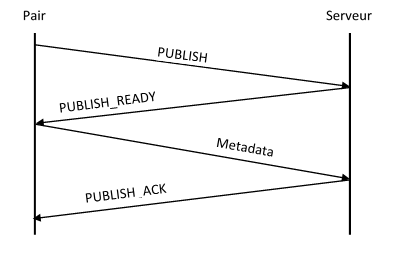
\includegraphics[scale=1]{Publish.png}
	\end{center}
	\caption{Protocole de publication}
	\label{publish}
\end{figure}

\subsection{Protocole de recherche (pair-serveur)}

Ce protocole est consultable sur la figure \ref{search}. Pour débuter l'échange, le client envoie une requête \texttt{SEARCH}. A nouveau, pour éviter de gêner l'écoute 
UDP avec d'autres messages, le serveur répond \texttt{SEARCH\_READY} depuis un port aléatoire généré par le système. Le client écrit alors au serveur sur ce port 
pour lui envoyer le mot-clef de recherche saisi par l'utilisateur. Le serveur recherche alors des torrents correspondant au mot-clef. Il renvoie alors au client 
le nombre de résultats à recevoir suivi de ces résultats (un par message) s'il en existe.

\begin{figure}
	\begin{center}
		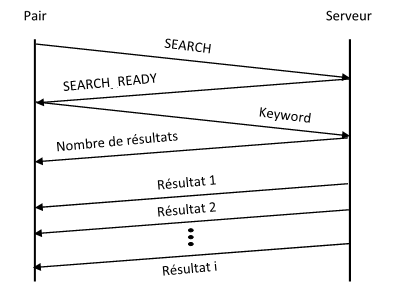
\includegraphics[scale=1]{Search.png}
	\end{center}
	\caption{Protocole de recherche}
	\label{search}
\end{figure}

\subsection{Protocole de récupération d'un fichier (pair-pair)}

Pour récupérer un fichier, le client commence par envoyer une requête \texttt{GET} suivie du SHA du fichier à récupérer sur le pair distant. Celui-ci recherche dans la liste 
des fichiers disponibles celui dont le SHA correspond à la valeur envoyée. S'il existe et est toujours disponible sur le disque, le serveur envoie le contenu au client. Il est 
découpé selon la limite du protocole TCP. Le protocole global est visible sur la figure \ref{get}.

\begin{figure}
	\begin{center}
		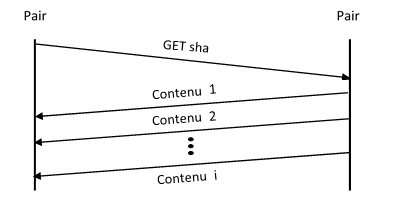
\includegraphics[scale=1]{Get.png}
	\end{center}
	\caption{Protocole de récupération d'un fichier}
	\label{get}
\end{figure}